\chapter[PROJETO E IMPLEMENTAÇÃO DO SERVIÇO DE PROCESSAMENTO]{PROJETO E IMPLEMENTAÇÃO DO SERVIÇO DE PROCESSAMENTO}

\label{chapter:architecture}

Escolhemos a \textbf{Arquitetura Kappa} como padrão de projeto para servir
de base para o novo serviço de processamento de dados do InterSCity.
A Arquitetura Lambda não justifica a maior complexidade no contexto atual da
plataforma, de modo que essa escolha facilita a manutenibilidade e adoção do
serviço pelo time atual do InterSCity. A Arquitetura Kappa permitirá a análise
em tempo-real sem que ocorra perda de informações relevantes, o que é
importante no contexto de cidades inteligentes, ao passo em que permite a
análise de dados históricos, desde que estes tenham sido pré-processados.
Esta decisão resulta na necessidade de escolha de uma tecnologia de
processamento \textit{streaming} e de um \textit{broker} adequado.

Escolhemos o \textbf{Apache Spark} como tecnologia de \textit{streaming}
a ser usada, principalmente por dispor nativamente de biblioteca de clusterização
e aprendizagem de máquina. Esta ferramenta ainda facilita, caso necessário, a
troca para a Arquitetura Lambda, por dispor de processamento \textit{batch}.
Escolhemos o \textbf{Apache Kafka} como o \textit{broker} do novo serviço de
processamento, sendo esta uma escolha menos óbvia que a anterior. Embora o
RabbitMQ já seja utilizado pelo InterSCity e tenha vantagens em certos aspectos
em relação ao Kafka, não dispor de uma interface nativa que o conecte ao Spark
resultou nessa decisão. Outro fator é o gerenciamento nativo de \textit{log}
por parte do Kafka, que ajuda na implantação da Arquitetura Kappa. O Kafka,
contudo, só será utilizado no serviço de processamento de dados, não forçando
mudanças no ecossistema de microsserviços do InterSCity.

A Figura \ref{fig:stack} ilustra a pilha de tecnologias que deve compor a
Arquitetura Kappa no InterSCity, e as principais relações entre os diferentes
serviços.

\begin{figure}
  \centering
    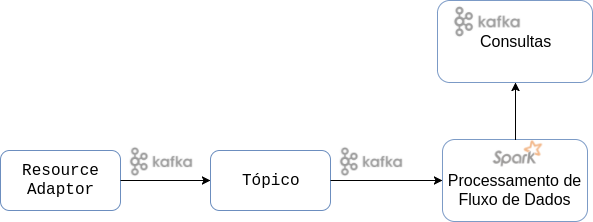
\includegraphics[scale=0.5]{figuras/kappa_tools2.png}
  \caption{Pilha de tecnologias utilizadas - Apache Kafka e Apache Spark, e suas
    interações com o InterSCity.}
  \label{fig:stack}
\end{figure}

\section{IMPLEMENTAÇÃO}

Dividimos a implementação da Arquitetura Kappa em três etapas:
(i) configuração do ambiente, contemplando as ferramentas escolhidas;
(ii) ligações entre os diferentes serviços, tornando possível a publicação de
    mensagens no Kafka e sendo possível seu processamento no Spark; e
(iii) disponibilização de \textit{hooks} que possam ser estendidos futuramente,
    possibilitando a criação de um \textit{pipeline de dados} customizável.

A implementação do novo serviço trouxe para o InterSCity o \textbf{Shock},
um componente responsável por abstrair as comunicações entre as diferentes
ferramentas e trazer a extensibilidade mencionada na terceira etapa da
implementação. Pseudo algoritmos presentes no Apêndice \ref{appendix:impl}
ilustram o uso das ferramentas escolhidas na implementação da Arquitetura
Lambda\footnote{
Pseudo códigos para a Arquitetura Lambda foram disponibilizados como forma
de complemento, pois o Shock já contempla a Arquitetura Kappa.
}.

\begin{figure}
  \centering
    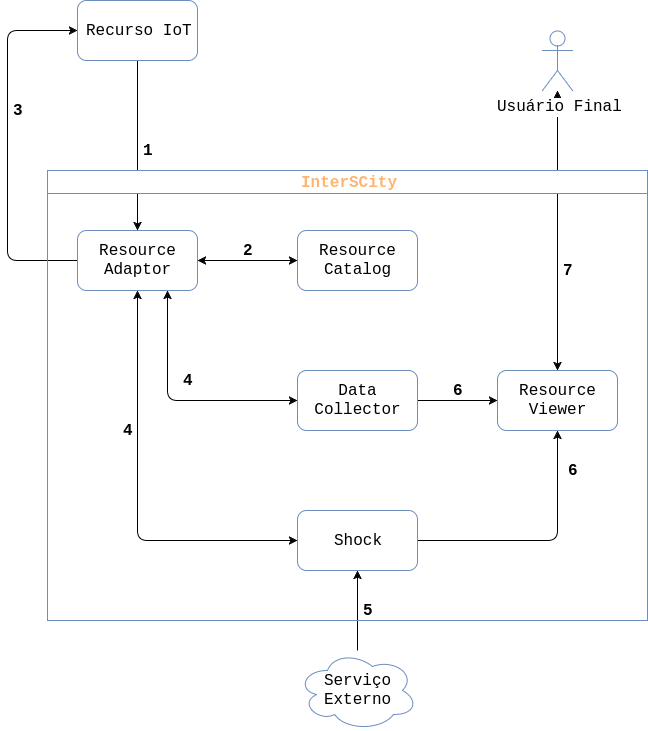
\includegraphics[scale=0.45]{figuras/shock_usage.png}
    \caption{Novo ciclo de vida da plataforma, com relação ao novo serviço de processamento.}
  \label{fig:shock_usage}
\end{figure}

A Figura \ref{fig:shock_usage} ilustra um novo fluxo completo do InterSCity
com a adição do novo serviço de processamento de dados. O início do fluxo
(passos 1 ao 3) continua o mesmo, e foi detalhado na Seção
\ref{sec:architecture}. As mudanças começam quando o (4) Resource Adaptor passa
a publicar a chegada de novos dados também no Shock através do Kafka, algo que
não trouxe grandes mudanças, mas que estendeu o InterSCity. Serviços externos
(5) anunciam no Shock quais operações devem ser executadas no \textit{stream}
de dados, de modo que os novos dados serão processados com esse conjunto de
operações. Por fim, os resultados do Shock e do Data Collector (6) serão
disponibilizados, podendo ser consumidos por aplicações como o microsserviço
Resource Viewer, que trata os dados para (7) disponibilizá-los ao usuário final.

A configuração do ambiente, assim como seguido pelo time do InterSCity, foi
guiada pelo uso de conteinêres do Docker. Reutilizamos uma configuração do
Spark que já havia sido desenvolvida pelo time do InterSCity, precisando de
poucas mudanças. Configuramos um conteinêr com o Kafka e o ligamos
aos conteinêres do Spark e do microsserviço Resource Adaptor.

A ligação entre os projetos teve início com uma adaptação no microsserviço
Resource Adaptor, que, com a mudança, passa a publicar em um tópico específico
no Kafka a atualização de novos dados. Essa adaptação não trouxe mudanças
significativas no InterSCity, não afetando o fluxo usual da plataforma.
Desenvolvemos então o Shock, responsável por receber mensagens em tópicos
específicos do Kafka e passá-los ao Spark Streaming. O Shock gerencia a
execução de \textit{micro-batches} do Spark em intervalos de tempos definidos
previamente, e em cada um destes processamentos, \textit{hooks} extensíveis são
executados. Caso queira-se anexar mais uma tarefa no
\textit{pipeline de dados}, basta então registrá-la no Shock e fornecer uma
prioridade, que define se uma tarefa deve ser executada antes ou depois.

\section{SHOCK}

O Shock se encontra disponível em um repositório no
Gitlab\footnote{\url{https://gitlab.com/DGuedes/shock}}, e o novo microsserviço
de processamento de dados pode ser encontrado em um \textit{fork} do serviço
original\footnote{\url{https://gitlab.com/DGuedes/data-processor}}. O Shock
abstrai as configurações entre as diferentes ferramentas e pode ser customizado
por serviços externos que definem quais operações devem ser executadas.
É configurável, possuindo um \textit{handler} para a Arquitetura Kappa
desenvolvido\footnote{\url{https://gitlab.com/DGuedes/shock/blob/master/shock/handlers.py}},
mas caso seja desejado a implementação de um outro \textit{handler}, basta
implementar as funções obrigatórias e fornecer o novo módulo como parâmetro
para o Shock.

\begin{figure}
  \centering
    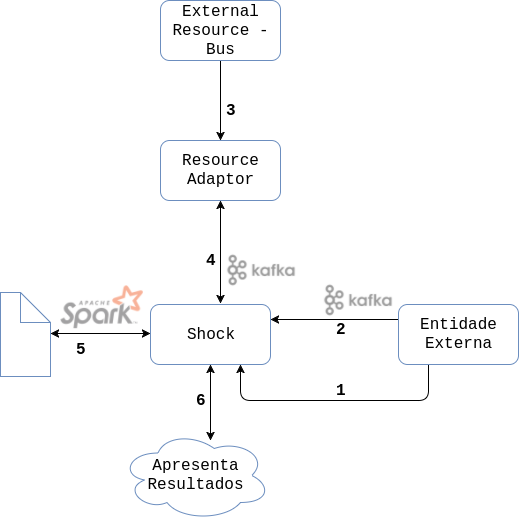
\includegraphics[scale=0.45]{figuras/shock.png}
    \caption{Ciclo de vida do Shock dentro do InterSCity.}
  \label{fig:shock}
\end{figure}

A Figura \ref{fig:shock} ilustra o uso do Shock, utilizando como exemplo uma
aplicação de cidades inteligentes desenvolvida pelo time do
InterSCity\footnote{\url{https://gitlab.com/smart-city-software-platform/external-resources/tree/master/bus}}.
Essa aplicação disponibiliza as coordenadas, tempo, o índice e a linha de alguns
ônibus de São Paulo. Imaginando que seja desejado a criação de uma nova informação
a partir destes dados, como a \textit{velocidade}, o fluxo de uso com o Shock
poderia ser: (1) uma
entidade\footnote{Entidade neste cenário se trata de qualquer serviço externo que deseje
contribuir com o InterSCity.} fornece ao Shock um arquivo contendo um conjunto
de funções necessárias para compor o \textit{pipeline de dados}. Essa etapa é
opcional, e o controle entre quem pode ou não enviar os arquivos desejados não
cabe ao Shock, e sim a quem tem acesso ao servidor. A entidade externa então
(2) constrói o \textit{pipeline de dados} através de publicações no Kafka, que
serão recebidos pelo Shock, transformando os \textit{streams} de processamento.
Os recursos IoT (3) publicam no Resource Adaptor a chegada de novos dados,
neste caso, sobre os ônibus. O Resource Adaptor (4) publica os novos dados em um
tópico específico no Kafka para que sejam recebidos pelo Shock, que os (5)
processa através do Spark no próximo \textit{micro-batch} escalonado, já
utilizando as funções registradas no passo 2. Por fim, após o processamento
dos dados, o Shock (6) disponibiliza os resultados do processamento.
